\documentclass{article}
\usepackage{amsmath}
\usepackage{amssymb}
\usepackage{amsbsy}
\usepackage{bm}
\usepackage{bbm}
\usepackage{url}
\usepackage{xcolor}
\usepackage{float}
\usepackage{graphicx}
\usepackage{epstopdf}
\usepackage{fancyhdr}
\usepackage{enumerate}
\usepackage{tikz}
\usepackage[ruled,vlined]{algorithm2e}
\usepackage[colorlinks=true,urlcolor=blue]{hyperref}
\usepackage[utf8]{inputenc}
\numberwithin{figure}{section}

\graphicspath{{assets/}}
\newcommand{\ent}[1]{\mathbf{#1}}
\newcommand{\rel}{\boldsymbol{\ell}}
\newcommand{\Solution}[1]{%
    {%
        \medskip
        \color{red}
        \bf $\bigstar$~\sf\textbf{Solution}~$\bigstar$ \sf
        #1
    }
    \bigskip
}

\title{CS224W Homework 2}
\date{Due: October 29, 2026}

\begin{document}
\maketitle

\section{GNNs as MLP of eigenvectors [20 points]}
\noindent \textit{Coverage: This problem is covered in Lecture 7.}

In this problem, we analyze message-passing GNN layers from a spectral perspective. We will (i) rewrite per-node updates in a batch matrix form, (ii) specialize to a single-layer MLP, and (iii) express the layer outputs in the eigenvector basis of the (symmetric) adjacency matrix.

\subsection{Batch Node Update [2 points]}
Consider the update for Graph Isomorphism Network (GIN):
\begin{equation}
\mathbf{x}_v^{(l+1)}=\operatorname{\texttt{MLP}}\left((1+\epsilon)\mathbf{x}_v^{(l)}+\sum_{u\in\mathcal{N}(v)}\mathbf{x}_u^{(l)}\right),
\end{equation}
where $\mathbf{x}_v^{(l)}\in\mathbb{R}^{d_l}$ is the embedding of node $v$ at layer $l$. Let $\textbf{X}^{(l)}\in\mathbb{R}^{N\times d_l}$ be a matrix containing the embeddings of all the nodes in the graph, i.e., $\textbf{X}^{(l)}[v,:]=\mathbf{x}_v^{(l)\top}$. Also, let $\textbf{A}\in\{0,1\}^{N\times N}$ represent the adjacency matrix of the graph. Write down the update of $\textbf{X}^{(l+1)}$ as a function of $\textbf{X}^{(l)}$ and $\textbf{A}$.

\Solution{}

\subsection{Single Layer MLP [2 points]}
Assume that \texttt{MLP}() represents a single layer MLP with no bias term followed by a pointwise nonlinearity $\sigma$. Write down the update of $\textbf{X}^{(l+1)}$ as a function of $\textbf{X}^{(l)}$ and $\textbf{A}$, and the trainable parameters $\textbf{W}^{(l)}$ of layer $l$.

\Solution{}

\subsection{Eigenvector Extension [4 points]}
Let $\{\lambda_n,\mathbf{v}_n\}_{n=1}^N$ represent the eigenvalues and eigenvectors of the symmetric adjacency $\textbf{A}$. Then we can write $\textbf{A}=\textbf{V}\mathbf{\Lambda} \textbf{V}^\top$, where $\textbf{V}\in\mathbb{R}^{N\times N}$ is the matrix of eigenvectors with $\textbf{V}[:,n]=\mathbf{v}_n$ and $\mathbf{\Lambda}\in\mathbb{R}^{N\times N}$ is the diagonal matrix of eigenvalues with $\mathbf{\Lambda}[n,n]=\lambda_n$. Show that
\[\textbf{X}^{(l+1)}=\sigma\left(\textbf{V}\mathbf{\hat W}^{(l)}\right)\]
where $\mathbf{\hat W}^{(l)}$ has entries
\[\mathbf{\hat W}^{(l)}[n,j]=(\lambda_n+1+\epsilon)\sum_{i=1}^{d_l}\textbf{W}^{(l)}[i,j]\left\langle\mathbf{v}_n,\textbf{X}^{(l)}[:,i]\right\rangle,\]
and $\langle\cdot\rangle$ denotes the dot product.

Hint: Use the fact that the eigenvectors of a symmetric matrix form an orthonormal basis. In other words, the matrix $\textbf{V}$ of eigenvectors is orthogonal, i.e., $\textbf{V}^\top \textbf{V}=\textbf{VV}^\top=\textbf{I}$. Next, show that each feature across all nodes, $\textbf{X}^{(l+1)}[:,i]$, can be expressed as a linear combination of eigenvectors, followed by a pointwise nonlinearity.

\Solution{}

\subsection{GraphSAGE [4 points]}
Perform the same analysis for the GraphSAGE update when the aggregation function is sum pooling, i.e., derive (i) $\textbf{X}^{(l+1)}$ and (ii) $\mathbf{\hat W}^{(l)}[n,j]$. Recall that the GraphSAGE update function is
\begin{align*}
\mathbf{x}_v^{(l+1)}&=\sigma\left(\textbf{W}^{(l)}\cdot\operatorname{CONCAT}\left(\mathbf{x}_v^{(l)},\mathbf{x}_{\mathcal{N}(v)}^{(l)}\right)\right)\\
&=\sigma\left(\textbf{W}_1^{(l)}\mathbf{x}_v^{(l)}+\textbf{W}_2^{(l)}\operatorname{AGG}\left(\mathbf{x}_u^{(l)},\ \forall u\in N(v)\right)\right).
\end{align*}
You may define the weight matrices using either the row-vector or column-vector convention, provided you specify their dimensions and use them consistently.

\subsection{Eigendecomposition Analysis [8 points]}
\begin{figure}[H]
\centering
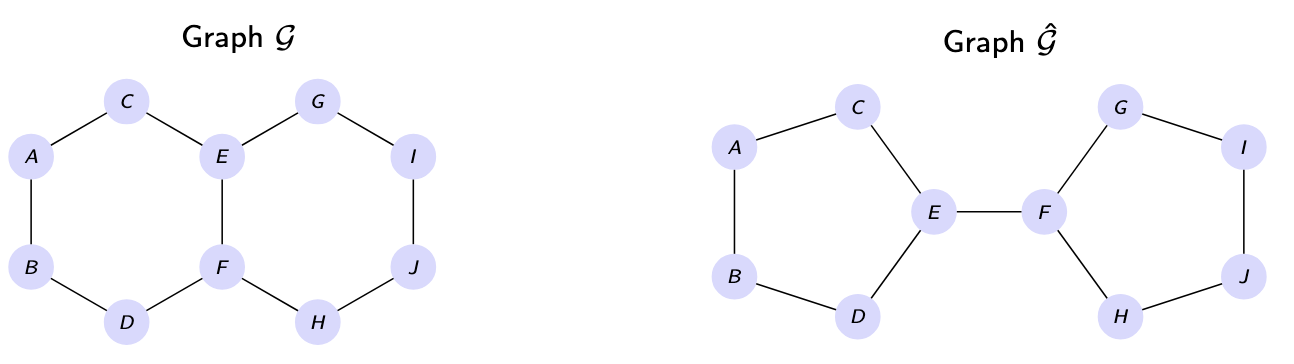
\includegraphics[width=0.75\textwidth]{eigendecomp_graph.png}
\end{figure}
\begin{enumerate}
\item For graphs $\mathcal{G}$ and $ \hat{\mathcal{G}}$ instantiate the graph adjacencies in Numpy, PyTorch, or PyG, and compute their eigenvalue decompositions. What do you observe? [2 points]

\Solution{}

\item Consider a GIN where all nodes start with the same initial color, i.e., $\mathbf{x}_v^{(0)}=1$ for all nodes $v\in \mathcal{V}$. This setup is equivalent to having $\textbf{X}^{(0)}=\mathbf{1}$, where $\mathbf{1}$ denotes the all-one vector. This is the initialization of the WL test. Using the equations in 1.3, derive the expression for $\textbf{X}^{(1)}$. [2 points]

\Solution{}

\item Observe from your previous result that each column $\textbf{X}^{(1)}[:,j]$ is a linear combination of eigenvectors, followed by a pointwise nonlinearity. What is the weight associated with each eigenvector? What factors determine this weight? [2 points]

\Solution{}

\item Compute the dot product $\langle\mathbf{v}_n,\textbf{X}^{(0)}\rangle$, for each eigenvector across both graphs. In other words, compute the dot products $c_n=\langle\mathbf{v}_n,\mathbf{1}_N\rangle$ for $\mathcal{G}$ and $\hat c_n=\langle\hat{\mathbf{v}}_n,\mathbf{1}_N\rangle$ for $\hat{\mathcal G}$. What do you observe? [1 point]

\Solution{}

\item What does the previous result suggest about $\textbf{X}^{(1)}$ for the graphs $\mathcal{G}$ and $\hat{\mathcal G}$? [1 point]

\Solution{}

\end{enumerate}


\section{Node Embeddings with TransE [21 points]}
\noindent \textit{Coverage: This problem is covered in Lecture 10.}

While many real world systems are effectively modeled as graphs, graphs can be a cumbersome format for certain downstream applications, such as machine learning models. It is often useful to represent each node of a graph as a vector in a continuous low dimensional space. The goal is to preserve information about the structure of the graph in the vectors assigned to each node. For instance, the spectral embedding preserved structure in the sense that nodes connected by an edge were usually close together in the (one-dimensional) embedding $x$.\\

\noindent Multi-relational graphs are graphs with multiple types of edges. They are incredibly useful for representing structured information, as in knowledge graphs. There may be one node representing “Washington, DC” and another representing “United States”, and an edge between them with the type “Is capital of”. In order to create an embedding for this type of graph, we need to capture information about not just which edges exist, but what the types of those edges are. In this problem, we will explore a particular algorithm designed to learn node embeddings for multi-relational graphs. \\\\
The algorithm we will look at is TransE.\footnote{See the 2013 NeurIPS paper by Bordes et al: \url{https://papers.nips.cc/paper/5071-translating-embeddings-for-modeling-multi-relational-data.pdf}}
We will first introduce some notation used in the paper describing this algorithm.
We’ll let a multi-relational graph $G = (E, S, L)$ consist of the set of \textit{entities} $E$ (i.e., nodes), a set of edges $S$, and a set of possible relationships $L$.
The set $S$ consists of triples $(h, l, t)$, where $h \in E$ is the \textit{head} or source-node, $l \in L$ is the relationship, and $t \in E$ is the \textit{tail} or destination-node.
As a node embedding, TransE tries to learn embeddings of each entity $e \in E$ into $\mathbb{R}^k$ ( $k$-dimensional vectors), which we will notate by $\mathbf{e}$. The main innovation of TransE is that each relationship $\ell$ is also embedded as a vector $\boldsymbol{\ell} \in \mathbb{R}^k$, such that the difference between the embeddings of entities linked via the relationship $\ell$ is approximately $\boldsymbol{\ell}$. That is, if $(h, \ell, t) \in S$, TransE tries to ensure that $\mathbf{h}+\boldsymbol{\ell} \approx \mathbf{t}$. Simultaneously, TransE tries to make sure that $\mathbf{h}+\boldsymbol{\ell} \not\approx \mathbf{t}$ if the edge $(h, \ell, t)$ does not exist.\\\\
\textbf{Note on notation}: we will use unbolded letters $e, \ell$, etc. to denote the entities and relationships in the graph, and bold letters $\mathbf{e}, \boldsymbol{\ell}$, etc., to denote their corresponding embeddings.
TransE accomplishes this by minimizing the following loss:
\begin{equation}\tag{7}\label{eq1}
\mathcal{L}=\sum_{(h, \ell, t) \in S}\left(\sum_{\left(h^{\prime}, \ell, t^{\prime}\right) \in S_{(h, \ell, t)}^{\prime}}\left[\gamma+d(\mathbf{h}+\boldsymbol{\ell}, \mathbf{t})-d\left(\mathbf{h}^{\prime}+\boldsymbol{\ell}, \mathbf{t}^{\prime}\right)\right]_{+}\right)
\end{equation}
Here $\left(h^{\prime}, \ell, t^{\prime}\right)$ are "corrupted" triplets, chosen from the set $S_{(h, \ell, t)}^{\prime}$ of corruptions of $(h, \ell, t)$, which are all triples where either $h$ or $t$ (but not both) is replaced by a random entity, and $\ell$ remains the same as the one in the original triplets. For this homework, assume corrupted triples are not members of the set of true triples $S$.
$$
S_{(h, \ell, t)}^{\prime}=\left\{\left(h^{\prime}, \ell, t\right) \mid h^{\prime} \in E\right\} \cup\left\{\left(h, \ell, t^{\prime}\right) \mid t^{\prime} \in E\right\}
$$
Additionally, $\gamma>0$ is a fixed scalar called the \textit{margin}, the function $d(\cdot, \cdot)$ is the Euclidean distance, and $[\cdot]_{+}$ is the positive part function (defined as $\max (0, \cdot)$). Finally, TransE restricts \textbf{all the entity embeddings to have length $1:\|\mathbf{e}\|_2=1$ for every $e \in E$.}\\
For reference, here is the TransE algorithm, as described in the original paper on page 3:
\begin{figure}[H]
    \centering
    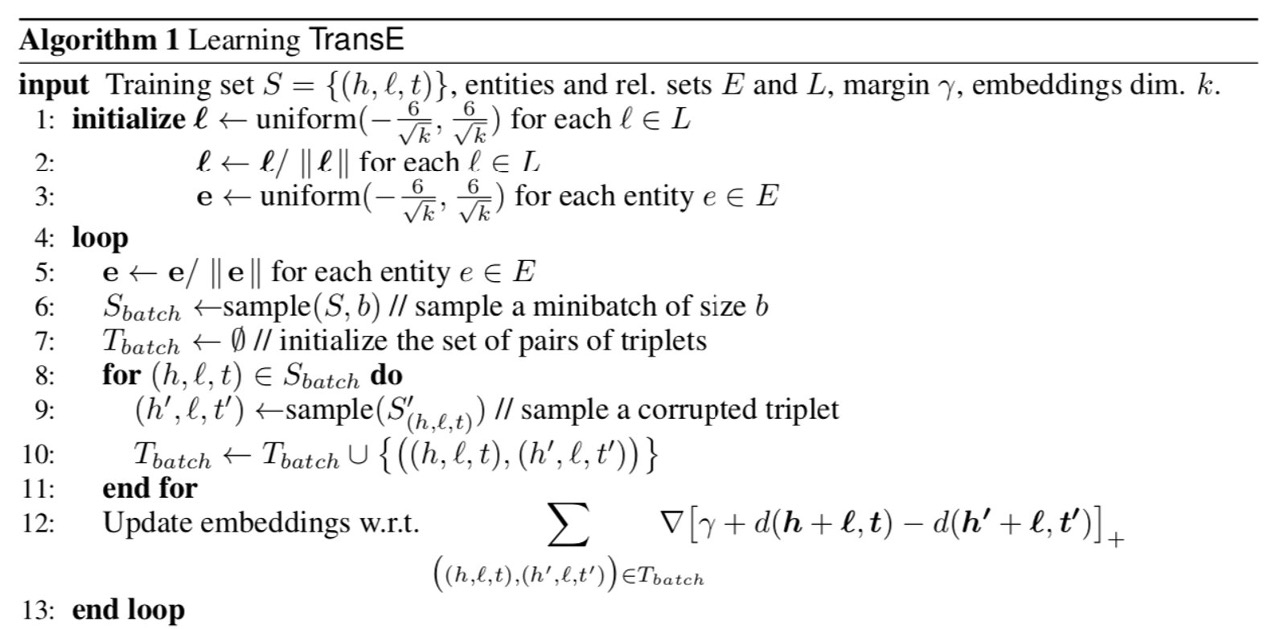
\includegraphics[width=1.0\textwidth]{algo2.png}
    \label{fig:algo2}
\end{figure}

\subsection{Simplified Objective [3 points]}
Say we were intent on using a simpler loss function. Our objective function (\ref{eq1}) includes a term maximizing the distance between $\mathbf{h}^{\prime}+\boldsymbol{\ell}$ and $\mathbf{t}^{\prime}$. If we instead simplified the objective, and just tried to minimize
\begin{equation}\tag{8}\label{eq2}
\mathcal{L}_{\text {simple }}=\sum_{(h, \ell, t) \in S} d(\mathbf{h}+\boldsymbol{\ell}, \mathbf{t}),
\end{equation}

we would obtain a useless embedding. Give an example of a simple graph and corresponding embeddings which will minimize the new objective function (\ref{eq2}) all the way to zero, but still give a completely useless embedding.\\
\textbf{Hint:} Your graph should be non-trivial, i.e., it should include at least two nodes and at least one edge. Assume the embeddings are in 2 dimensions, i.e., $k = 2$.
What happens if $\boldsymbol{\ell} = \textbf{0}$?

\Solution{}

\subsection{Utility of $\gamma$  [5 points]}
We are interested in understanding what the margin term $\gamma$ accomplishes. If we removed the margin term $\gamma$ from our loss, and instead optimized
\begin{equation}\tag{9}\label{eq3}
\mathcal{L}_{\text {no margin }}=\sum_{(h, \ell, t) \in S} \sum_{\left(h^{\prime}, \ell, t^{\prime}\right) \in S_{(h, \ell, t)}^{\prime}}\left[d(\mathbf{h}+\boldsymbol{\ell}, \mathbf{t})-d\left(\mathbf{h}^{\prime}+\boldsymbol{\ell}, \mathbf{t}^{\prime}\right)\right]_{+},
\end{equation}
it turns out that we would again obtain a useless embedding. Give an example of a simple graph and corresponding embeddings which will minimize the new objective function (\ref{eq3}) all the way to zero, but still give a completely useless embedding. By useless, we mean that in your example, you cannot tell just from the embeddings whether two nodes are linked by a particular relation (Note: your graph should be non-trivial, i.e., it should include at least two nodes and at least one edge. Assume the embeddings are in 2 dimensions, i.e., $k=2$.)

\Solution{}

\subsection{ Normalizing the embeddings [5 points]}
Recall that TransE normalizes every entity embedding to have unit length (see line 5 of the algorithm). The quality of our embeddings would be much worse if we did not have this step. To understand why, imagine running the algorithm with line 5 omitted. What could the algorithm do to trivially minimize the loss in this case? What would the embeddings it generates look like?

\Solution{}

\subsection{Expressiveness of TransE embeddings [8 points]}
Give an example of a simple graph for which no perfect embedding exists, i.e., no embedding perfectly satisfies $\mathbf{u}+\boldsymbol{\ell}=\mathbf{v}$ for all $(u, \ell, v) \in S$ and $\mathbf{u}+\boldsymbol{\ell} \neq \mathbf{v}$ for $(u, \ell, v) \notin S$, for any choice of entity embeddings ($\mathbf{e}$ for $e \in E$ ) and relationship embeddings ( $\boldsymbol{\ell}$ for $\ell \in L$ ). Explain why this graph has no perfect embedding in this system, and what that means about the expressiveness of TransE embeddings. As before, assume the embeddings are in 2 dimensions $(k=2)$.\\
\textbf{Hint:} Note that the condition for this question is slightly different from that for Question 2.1 and what we ask you to answer is different as well.

\Solution{}

\section{Expressive Power of Knowledge Graph Embeddings [10 points]}
TransE is a common method for learning representations of entities and relations in a knowledge graph. Given a triplet $(h, \ell, t)$, where entities embedded as $h$ and $t$ are related by a relation embedded as $\ell$, TransE trains entity and relation embeddings to make $h+\ell$ close to $t$. There are some common patterns that relations form:
\begin{itemize}
    \item Symmetry: A is married to B, and B is married to A.
    \item Inverse: A is teacher of B, and B is student of A. Note that teacher and student are 2 different relations and have their own embeddings.
    \item Composition: $\mathrm{A}$ is son of $\mathrm{B} ; \mathrm{C}$ is sister of $\mathrm{B}$, then $\mathrm{C}$ is aunt of $\mathrm{A}$. Again note that son, sister, and aunt are 3 different relations and have their own embeddings.
\end{itemize}
Unlike Question 2.4, Questions 3.1-3.3 only require satisfying
the embedding equations for true triples, excluding zero
translations or identity rotations.

\Solution{}

\subsection{TransE Modeling [3 points]}
For each of the above relational patterns, can TransE model it perfectly, such that $h+\ell=t$ for all relations? Explain why or why not. Note that here $\mathbf{0}$ embeddings for relation are undesirable since that means two entities related by that relation are identical and not distinguishable.

\Solution{}

\subsection{RotatE Modeling [3 points]}
Consider a new model, RotatE. Instead of training embeddings such that $h+\ell \approx t$, we train embeddings such that $h \circ \ell \approx t$. Here $\circ$ means rotation. You can think of $h$ as a vector of dimension $2 d$, representing $d$ $2 \mathrm{D}$ points. $\ell$ is a $d$-dimensional vector specifying rotation angles. When applying $\circ$, For all $i \in 0 \ldots d-1, \left(h_{2 i}, h_{2 i+1}\right)$ is rotated clockwise by $l_i$. Similar to TransE, the entity embeddings are also normalized to L2 norm 1. Can RotatE model the above 3 relation patterns perfectly? Why or why not?

\Solution{}

\subsection{Failure Cases [4 points]}
Give an example of a graph that RotatE cannot model. Can TransE model this graph?

\Solution{}


\section{Honor Code [0 points]}
(X) I have read and understood Stanford Honor Code before I submitted my
work.

**Collaboration: Write down the names \& SUNetIDs of students you collaborated with on Homework 2 (None if you didn’t).**

**Note: Read our website on our policy about collaboration!**

\end{document}

